\chapter{DESAIN DAN IMPLEMENTASI}
\label{chap:desainimplementasi}

% Ubah bagian-bagian berikut dengan isi dari desain dan implementasi

Pada bab ini akan dijelaskan mengenai bagaimana cara sistem bekerja sehingga menghasilkan output yang diinginkan. Sistem dibuat bertujuan untuk membuat model klasifikasi menggunakan support vertor machine sebagai alat yang akan mempelajari data input dan membuat model klasifikasi tingkat kantuk dengan menggunakan parameter PERCLOS dan MAR.

\section{Metode yang digunakan}
\label{sec:Metode} 


% Contoh input gambar dengan format *.jpg
\begin{figure} [H] \centering
  % Nama dari file gambar yang diinputkan
  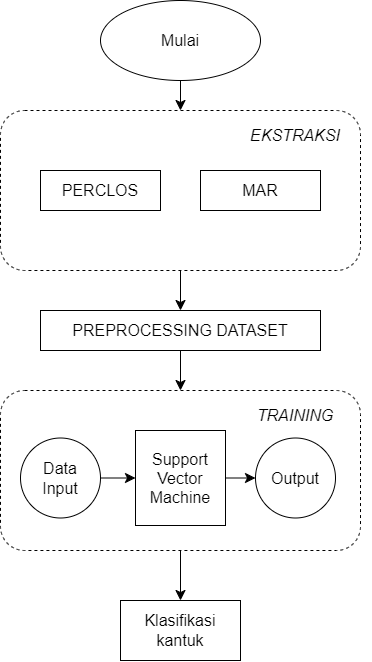
\includegraphics[scale=0.45]{gambar/2_2_7.png}
  % Keterangan gambar yang diinputkan
  \caption{Diagram Alur model}
  % Label referensi dari gambar yang diinputkan
  \label{fig:Diagram}
\end{figure}

% Contoh penggunaan referensi dari gambar yang diinputkan
Pada \emph{Diagram} yang tertera di Gambar \ref{fig:Diagram}. Akan digunakan metode seperti berikut :

\subsection{Pengumpulan Dataset}

Dalam penggunaan dataset,diperlukan beberapa kriteria sebagai input data yang kemudian nantinya akan diolah. Pada penelitian kali ini, akan digunakan dataset yang telah terverifikasi yaitu UTA-RLDD dataset. Data yang digunakan mempunyai durasi yang cukup untuk digunakan sebagai dataset. Kemudian dataset UTA-RLDD memiliki berbagai objek yang berbeda baik itu dari wajah, jenis kelamin, atau etnis. Data yang digunakan merupakan video yang memiliki fps rata-rata sekitar 30 FPS. Dataset UTA-RLDD akan digunakan untuk data testing dari model yang akan dibuat. Kemudian selain itu digunakan juga dataset DROZY. Dataset ini nantinya akan dilakukan ekstraksi nilai PERCLOS dan MAR dan kemudian diolah sehingga menghasilkan model yang diinginkan. 


\begin{figure} [H] \centering
  % Nama dari file gambar yang diinputkan
  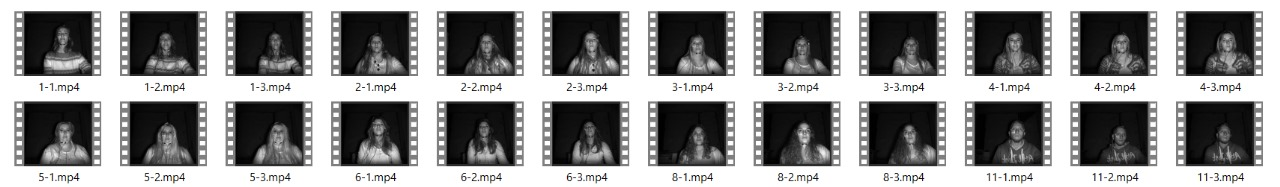
\includegraphics[scale=0.4]{gambar/3_1_4.jpg}
  % Keterangan gambar yang diinputkan
  \caption{Kumpulan Dataset}
  % Label referensi dari gambar yang diinputkan
  \label{fig:DatasetPic}
\end{figure}

\subsection{Preprocessing Dataset}
\label{subsec:Preprocessing}
\begin{enumerate}
  \item{\textbf{Interpolasi Frame Dataset}}
  
  Interpolasi frame Dataset dalam penelitian ini adalah video, merupakan teknik yang digunakan untuk meningkatkan jumlah frame per detik (FPS) dari sebuah video, sehingga menghasilkan pemutaran yang lebih halus. Salah satu metode yang umum digunakan untuk interpolasi frame video adalah melalui penggunaan encoder. Encoder bekerja dengan menambahkan frame baru antara frame asli video, menggunakan algoritma interpolasi untuk memperkirakan posisi objek dan piksel di antara frame asli tersebut. Hal ini sering dilakukan dengan bantuan perangkat keras khusus atau software yang mendukung pemrosesan video secara efisien.

  \begin{figure} [H] \centering
    % Nama dari file gambar yang diinputkan
    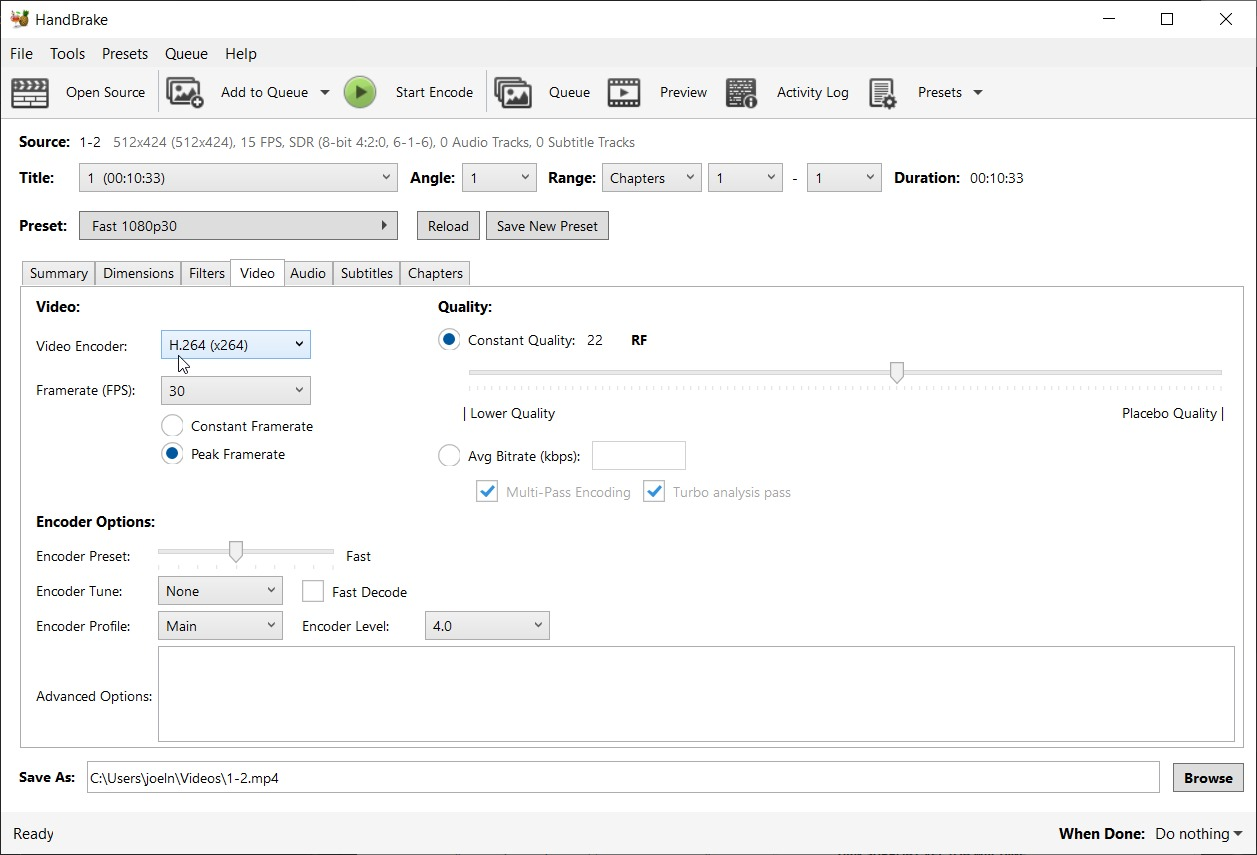
\includegraphics[scale=0.2]{gambar/Handbrake.jpg}
    % Keterangan gambar yang diinputkan
    \caption{HandBrake}
    % Label referensi dari gambar yang diinputkan
    \label{fig:HandBrake}
  \end{figure}

Salah satu software populer yang dapat digunakan untuk interpolasi frame video adalah HandBrake. HandBrake adalah alat open-source yang kuat untuk mengonversi dan memproses video, termasuk kemampuan untuk mengubah frame rate video. Dengan HandBrake, pengguna dapat meningkatkan FPS video dengan cara mengonfigurasi pengaturan encoding. Dalam proses ini, HandBrake menggunakan teknik interpolasi frame untuk menambahkan frame tambahan, menghasilkan video dengan frame rate yang lebih tinggi dan pemutaran yang lebih mulus. Prosesnya dimulai dengan membuka file video dalam HandBrake dan memilih preset yang sesuai atau mengonfigurasi pengaturan secara manual. Pengguna dapat mengatur frame rate target yang diinginkan, misalnya dari 15 FPS menjadi 30 FPS. HandBrake kemudian menggunakan encoder untuk melakukan interpolasi, menambahkan frame baru di antara frame yang sudah ada berdasarkan algoritma interpolasi yang dipilih. Setelah pengaturan selesai, proses encoding dimulai, dan HandBrake menghasilkan file video baru dengan frame rate yang lebih tinggi.

\begin{figure}[htbp]
  \centering
  \subfigure[FPS sebelum Interpolasi]{
    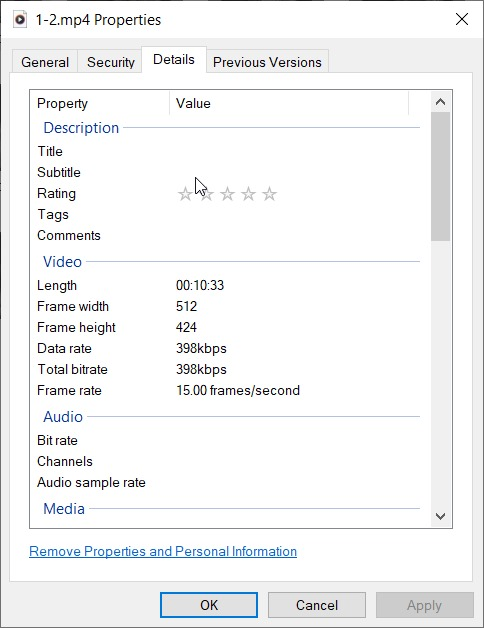
\includegraphics[scale=0.5]{gambar/Hasil1.jpg}
    \label{fig:FPS}
  }
  \hspace{0.5cm}
  \subfigure[FPS sesudah Interpolasi]{
    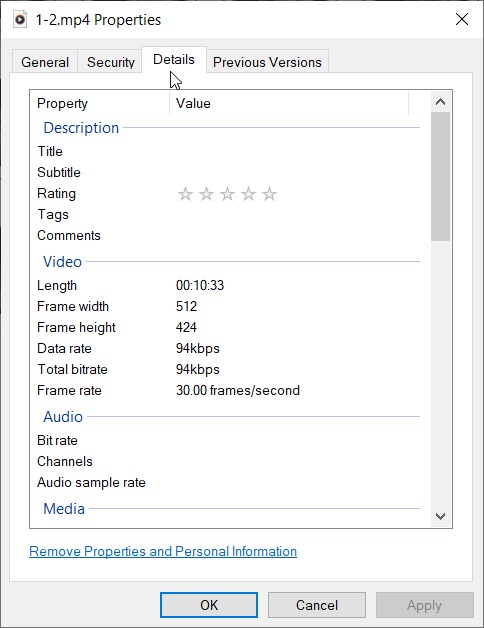
\includegraphics[scale=0.5]{gambar/hasil2.jpg}
    \label{fig:FPS2}
  }
  \caption{Perbandingan FPS sebelum dan sesudah interpolasi}
  \label{fig:FPS_comparison}
\end{figure}

  \item {\textbf{Landmark Dataset}}
  
  Pada proses deteksi fitur wajah dalam video yang dilakukan dengan PyCharm dan library Dlib, digunakan pendekatan deteksi landmark wajah melalui Histogram of Oriented Gradients (HOG) dan Support Vector Machine (SVM). Metode ini memberikan hasil identifikasi wajah yang akurat dalam video. Proses dimulai dengan deteksi wajah menggunakan HOG, yang merupakan teknik ekstraksi fitur yang kuat dalam mengenali wajah dengan berbagai orientasi dan kondisi pencahayaan. HOG bekerja dengan menghitung orientasi gradien di area gambar dan membuat histogram untuk mewakili distribusi gradien tersebut. Selanjutnya, SVM digunakan untuk mengklasifikasikan area yang mengandung wajah berdasarkan fitur HOG yang diekstraksi. SVM sangat efektif dalam membedakan antara wajah dan non-wajah karena kemampuannya untuk menemukan hyperplane optimal yang memisahkan dua kelas.

Setelah wajah terdeteksi, prediktor landmark dari Dlib digunakan untuk mengenali dan memetakan titik-titik penting pada wajah. Dlib menyediakan model pra-terlatih yang dapat mengenali 68 titik landmark pada wajah, mencakup area seperti mata, alis, hidung, mulut, dan kontur wajah. Proses ini melibatkan regresi ensemble yang memprediksi lokasi landmark berdasarkan citra input, memberikan koordinat yang presisi untuk setiap titik landmark. Dengan menggunakan 68 titik landmark ini, kita dapat melakukan berbagai analisis wajah lebih lanjut. Contohnya, koordinat dari landmark mata digunakan untuk menghitung Eye Aspect Ratio (EAR), yang merupakan indikator untuk mendeteksi kondisi mata tertutup atau terbuka. Selain itu, koordinat dari landmark mulut digunakan untuk menghitung Mouth Aspect Ratio (MAR), yang mengukur lebar dan tinggi mulut untuk mendeteksi ekspresi wajah seperti senyum atau menguap.

\begin{figure} [H] \centering
  % Nama dari file gambar yang diinputkan
  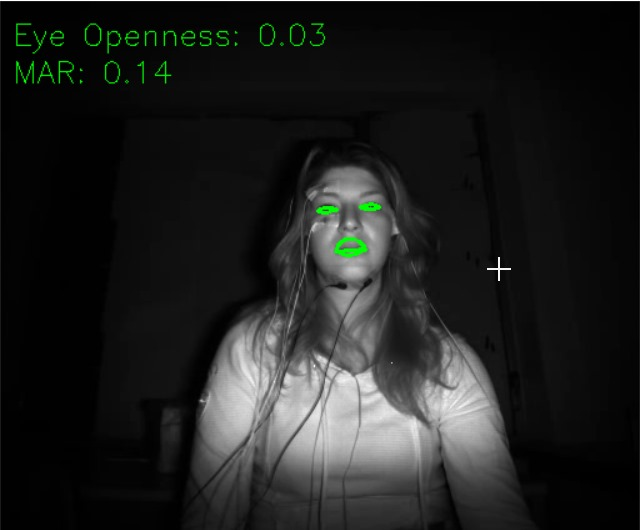
\includegraphics[scale=0.5]{gambar/3_1_2.jpg}
  % Keterangan gambar yang diinputkan
  \caption{Landmark Wajah}
  % Label referensi dari gambar yang diinputkan
  \label{fig:LandmarkW}
\end{figure}


  \item {\textbf{Ekstraksi Bukaan Mata dan Mulut}}
  
  \textbf{a. Deteksi Mata Kanan dan Mata Kiri}

  Setelah wajah terdeteksi, model prediktor landmark dari Dlib digunakan untuk mengenali dan memetakan titik-titik penting pada wajah. Dlib menyediakan model yang dapat mengenali 68 titik landmark pada wajah, mencakup area seperti mata, alis, hidung, mulut, dan kontur wajah. Dalam konteks ekstraksi mata, titik-titik landmark yang relevan adalah Mata Kiri: Titik 36 hingga 41. Mata Kanan: Titik 42 hingga 47.

Titik-titik ini memetakan kontur mata secara akurat. Untuk visualisasi, mata kiri biasanya digambarkan dengan warna hijau, sedangkan mata kanan digambarkan dengan warna merah, seperti yang terlihat pada gambar. Warna-warna ini membantu dalam membedakan antara mata kiri dan kanan dengan jelas. Proses selanjutnya melibatkan penggunaan koordinat dari titik-titik landmark tersebut untuk menggambar kontur di sekitar mata. Kontur ini digambar menggunakan fungsi dari OpenCV yang memungkinkan visualisasi yang jelas dari area mata.

\begin{figure} [H] \centering
  % Nama dari file gambar yang diinputkan
  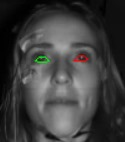
\includegraphics[scale=1.65]{gambar/mata.jpg}
  % Keterangan gambar yang diinputkan
  \caption{Landmark mata}
  % Label referensi dari gambar yang diinputkan
  \label{fig:Landmarkmata}
\end{figure}

  \textbf{b. Hitung Luasan Mata dan Mulut}

  Gambar 3.6 menunjukkan area yang ditandai hanya pada mata. Hal ini dilakukan sehingga hanya area mata yang dibutuhkan pada wajah untuk penelitian ini. Selanjutnya, area mata ini yang difokuskan, sehingga melalui koordinat yang ada, mata kanan dan mata kiri dapat dipisah atau dipotong. Setelah dipotong, setiap mata dibuat menjadi citra binary, sehingga hanya tersisa warna hitam dan putih. Gambar 3.7 menunjukkan mata yang telah dipotong dan dibuat ke binary.

  \begin{figure}[htbp]
    \centering
    \subfigure[left Eye]{
      
\includegraphics[scale=5]{gambar/lefteye.jpg}
      \label{fig:left}
    }
    \hspace{0.5cm}
    \subfigure[Right Eye]{
      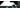
\includegraphics[scale=5]{gambar/righteye.jpg}
      \label{fig:right}
    }
    \caption{Binary Eye}
    \label{fig:Binary_eye}
  \end{figure}
  

Mata yang dibuat ke binary ini dilakukan masking agar area yang berwarna hitam hanya pada mata dan sekitarnya berwarna putih. Gambar 3.7 menunjukkan hanya mata saja yang berwarna putih. Hal ini dibutuhkan untuk dilanjutkan ke tahap berikutnya, yaitu mencari luas berdasarkan piksel berwarna putih. Setelah sampai pada tahap masking mata, seperti pada Gambar 3.7, maka tahap selanjutnya adalah mendapatkan luas mata. Luas mata dapat dihitung dengan menjumlahkan semua piksel yang berwarna putih. Berdasarkan hal ini, maka apabila mata seseorang terbuka, maka area berwarna putih juga akan meluas, sebaliknya, apabila mata seseorang tertutup, maka luas mata yang berwarna putih akan mengecil.

Perhitungan nilai Openness dilakukan dengan membandingkan jumlah piksel berwarna putih pada citra mata binary terhadap total piksel pada citra tersebut. Nilai Openness memberikan indikasi seberapa terbuka mata seseorang dalam frame tersebut. Sedangkan, Mouth Aspect Ratio (MAR) dihitung menggunakan koordinat dari titik-titik landmark pada mulut, dengan rumus yang memperhitungkan jarak antara titik-titik tertentu di bagian atas dan bawah serta sisi-sisi mulut. MAR memberikan indikasi tentang ekspresi wajah, seperti menguap atau berbicara.

\begin{figure} [H] \centering
  % Nama dari file gambar yang diinputkan
  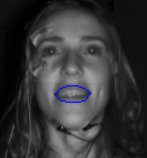
\includegraphics[scale=1.65]{gambar/mouth.jpg}
  % Keterangan gambar yang diinputkan
  \caption{Landmark mulut}
  % Label referensi dari gambar yang diinputkan
  \label{fig:Landmarkmulut}
\end{figure}

  \textbf{c. Interpolasi Data Luas Mata dan Mulut}

Pada proses ini, dilakukan optimasi pada hasi data yang didapatkan. Karena saat pemrosesan video, ada frame-frame yang tidak terdeteksi landmark-nya sehingga membuat data Openness dan MAR menjadi 0, diperlukan optimasi agar data yang hilang tersebut dapat direkonstruksi secara sintetis. Optimasi atau rekonstruksi ini dilakukan dengan menggunakan metode interpolasi. Pada penelitian ini digunakan interpolasi linear, di mana data yang diinterpolasi adalah hasil ekstraksi nilai Openness dan MAR.

Interpolasi linear adalah metode yang sederhana dan efektif untuk memperkirakan nilai-nilai di antara dua titik data yang diketahui. Dalam konteks ini, jika data Openness dan MAR pada frame tertentu tidak terdeteksi (bernilai 0), nilai tersebut diganti menjadi NaN (Not a Number). Kemudian, interpolasi linear digunakan untuk mengisi nilai-nilai NaN tersebut. Proses interpolasi linear bekerja dengan menggambar garis lurus antara dua titik data yang diketahui dan menggunakan garis tersebut untuk memperkirakan nilai di antara kedua titik. Dengan menggunakan interpolasi linear, nilai-nilai Openness dan MAR yang hilang dapat diisi dengan nilai yang logis dan konsisten dengan perubahan asli, menghasilkan transisi yang halus antara nilai tiap frame dan meningkatkan fluiditas hasil analisis video. Teknik ini membantu mengatasi masalah data yang hilang akibat deteksi landmark yang tidak sempurna, memastikan bahwa analisis tetap akurat dan andal.
\end{enumerate}

\subsection{Hitung data PERCLOS dan MAR}
\label{subsec:HitungPERCLOS}
 Berdasarkan penelitian \parencite{7545182}. Untuk mendapatkan nilai PERCLOS, pertama sekali diperlukan nilai treshold untuk menentukan nilai acuan untuk menentukan apakah kondisi mata sedang terbuka atau tertutup. Untuk mencari treshold ditentukan diurutkan data mulai dari tertinggi sampai pada data yang bernilai terendah. Pengurutan data ini dilakukan kepada tiap data atau file csv yang berisi nilai bukaan mata sebelumnya. Sehingga, nilai treshold yang dimiliki tiap data atau tiap file csv memiliki nilai yang berbeda.

 Setelah data diurutkan, kemudian dilakukan perhitungan rata rata untuk mendapatkan nilai rata rata O dan C. Untuk mendapatkan nilai O, dilakukan perhitungan 1/20 total data. Hasil dari nilai 1/20 total data ini digunakan untuk mengambil data teratas sebanyak hasil 1/20 total data sebelumnya dan kemudian dirata ratakan untuk mendapatkan nilai O. Sebaliknya, dari data paling rendah diambil sebanyak 1/20 total data dan kemudian dirata ratakan untuk mendapatkan nilai C. Setelah itu dilakukan perhitungan treshold dengan menggunakan rumus 3.1.

 \begin{equation}
  Threshold = (O - C)* 0,2 + C
\end{equation}


Kemudian setelah didapatkan nilai treshold nya, semua data yang berada di atas treshold dikelompokkan per 30 frame data. Sehingga total nilai nya dianggap sebagai nIO, sedangkan data yang bernilai dibawah treshold dikelompokkan per 30 frame data,dijumlahkan dan dianggap sebagai nIC. Setelah masing masing nilai didapat, maka nilai PERCLOS bisa didapat. Untuk rumus PERCLOS dapat dilihat pada rumus 3.2. 

\begin{equation}
\label{eq:PERCLOSeq}
  PERCLOS = \frac{\emph{nIC} }{\emph{nIC} + \emph{nIO}}
\end{equation}

Perhitungan ini dilakukan terhadap semua file csv yang berisi data bukaan mata. Sehingga total data PERCLOS yang didapatkan berbeda pula.

Sedangkan untuk perhitungan nilai MAR, digunakan rumus 2.2. Titik-titik landmark diperoleh dari model prediktor landmark wajah, seperti yang disediakan oleh Dlib. Penghitungan jarak Euclidean antara titik-titik ini memberikan ukuran yang digunakan untuk menghitung MAR. Dengan kata lain, MAR adalah perbandingan antara lebar vertikal dan horizontal mulut, memberikan indikator yang dapat digunakan untuk analisis ekspresi wajah. Nilai MAR yang tinggi menunjukkan bahwa mulut lebih terbuka, yang bisa mengindikasikan menguap atau berbicara, sedangkan nilai yang lebih rendah menunjukkan mulut yang lebih tertutup. 

\begin{lstlisting}[
  language=Python,
  caption={Menghitung PERCLOS.},
  label={lst:PERCLOS}
]
import pandas as pd

def calculate_threshold(chunk):
    """
    Hitung threshold untuk chunk data.
    """
    total_frames = len(chunk)
    A = total_frames // 20
    A = max(A, 1)

    sorted_data = chunk.sort_values(by='EAR', ascending=False)

    O = sorted_data['EAR'].head(A).mean()
    C = sorted_data['EAR'].tail(A).mean()

    threshold = (O - C) * 0.2 + C

    return threshold

def process_data(file_path):
    df = pd.read_csv(file_path)
    if 'EAR' not in df.columns or 'MAR' not in df.columns:
        raise ValueError("Kolom 'EAR' atau 'MAR' tidak ditemukan dalam file CSV")
    
    result = []

    for i in range(0, len(df), 30):
        chunk = df.iloc[i:i+30]
        
        if len(chunk) == 0:
            continue
        
        threshold = calculate_threshold(chunk)

        chunk_openness = chunk['EAR']
        chunk_mar = chunk['MAR']

        above_threshold = chunk_openness[chunk_openness > threshold]
        below_threshold = chunk_openness[chunk_openness <= threshold]
        
        sum_above = above_threshold.sum()
        sum_below = below_threshold.sum()

        std_mar = chunk_mar.std()
        
        result.append({
            'Sum_Above_Threshold': sum_above,
            'Sum_Below_Threshold': sum_below,
            'MAR_Std': std_mar
        })

    result_df = pd.DataFrame(result)
    
    return result_df

def calculate_ratio(data):
    data['PERCLOS'] = data['Sum_Below_Threshold'] / (data['Sum_Above_Threshold'] + data['Sum_Below_Threshold'])
    
    result_df = data[(data['PERCLOS'] > 0) & (data['PERCLOS'] < 0.8)]
    result_df = result_df[['PERCLOS', 'MAR_Std']]
    
    return result_df

file_path = r'F:\SKRIPSI\TA\Fix_code\SkripSHYs\DataEARMAR\14-3_data_analysis.csv'
final_output_path = r'F:\SKRIPSI\TA\Fix_code\SkripSHYs\PERCLOS\Perclos\14-3_final_result.csv'

processed_data = process_data(file_path)
final_result = calculate_ratio(processed_data)
final_result.to_csv(final_output_path, index=False)

print(f"Proses selesai. Hasil disimpan di {final_output_path}")


\end{lstlisting}




\subsection{Labeling Data}
\label{subsec:Labelling}

Dalam tahapan preprocessing, proses labeling merupakan langkah krusial setelah interpolasi frame. Labeling melibatkan pengkategorian data berdasarkan karakteristik tertentu untuk memudahkan proses training. Sebelum data di training tentunya data harus diberikan label agar nantinya data tersebut dapat dikenali dan dipelajari oleh machine learning. Proses ini bertujuan untuk menandai frame-frame dalam dataset video dengan label yang menunjukkan informasi tertentu, seperti tingkat keaktifan, ekspresi wajah, atau indikator kantuk pada subjek yang diamati. Dalam penelitian ini, labeling digunakan untuk memberikan informasi kelas kantuk yang dimiliki oleh data yang kita akan gunakan. Keakuratan dalam labeling secara langsung mempengaruhi kualitas hasil analisis menggunakan model pembelajaran mesin. Kesalahan dalam labeling dapat mengarah pada pembelajaran yang salah oleh model, yang pada akhirnya menurunkan performa model saat digunakan dalam pengujian nyata atau implementasi.

\begin{figure} [H] \centering
  % Nama dari file gambar yang diinputkan
  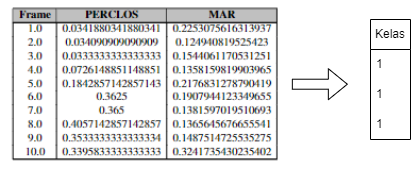
\includegraphics[scale=0.75]{gambar/label.png}
  % Keterangan gambar yang diinputkan
  \caption{Labelling }
  % Label referensi dari gambar yang diinputkan
  \label{fig:labell}
\end{figure}


\subsection{Balancing Data}
\label{subsec:Balancing}

Pada bagian ini akan dilakukan penyeimbangan data. Balancing data, atau penyeimbangan data, merupakan proses mengatasi permasalahan imbalance dalam dataset, yaitu ketika jumlah sampel untuk setiap kelas dalam data tidak seimbang. Fungsi balancing data adalah untuk meningkatkan kinerja model dengan memastikan bahwa setiap kelas diwakili secara adil dalam proses training
Dengan memastikan bahwa data untuk setiap kelas seimbang, model dapat belajar fitur dari setiap kelas secara lebih efektif, yang pada gilirannya dapat meningkatkan akurasi dan kinerja model secara keseluruhan.

Beberapa metode populer untuk balancing data meliputi:

Oversampling: Meningkatkan jumlah sampel dalam kelas minoritas dengan cara membuat duplikat sampel yang ada atau menambahkan sampel sintetis (misalnya, menggunakan teknik SMOTE - Synthetic Minority Over-sampling Technique).

Undersampling: Mengurangi jumlah sampel dalam kelas mayoritas untuk mencocokkan jumlah sampel di kelas minoritas. Metode ini bisa mengurangi informasi karena menghilangkan sampel dari dataset.

Pada tahap ini, diterapkan metode SMOTE (Synthetic Minority Over-sampling Technique) untuk penyeimbangan data.  Neighbors (KNN) untuk memilih sampel minoritas terdekat, kemudian menciptakan sampel baru di sepanjang garis yang menghubungkan sampel minoritas yang dipilih. Dengan cara ini, SMOTE dapat meningkatkan jumlah sampel dalam kelas minoritas secara lebih efektif dan realistis, sehingga membantu model belajar fitur dari kelas minoritas dengan lebih baik. Penerapan SMOTE dalam tahap ini membantu memastikan bahwa dataset yang digunakan untuk training model memiliki representasi yang seimbang dari setiap kelas. Hal ini sangat penting dalam situasi di mana ada perbedaan besar antara jumlah sampel kelas mayoritas dan minoritas, yang jika tidak ditangani, dapat menyebabkan model menjadi bias dan kurang akurat dalam memprediksi kelas minoritas.

\subsection{Data Model}
\label{subsec:datamodel}

Setelah dilakukan balancing data, didapatkan jumlah data yang diharapkan siap untuk dilakukan training. Setelah balancing dilakukan, bentuk dari data yang akan ditraining juga disesuaikan agar dapat dibaca dengan baik oleh kernel yang akan digunakan untuk melatih data. Pada tabel

% Please add the following required packages to your document preamble:
% \usepackage{booktabs}
% \usepackage[table,xcdraw]{xcolor}
% Beamer presentation requires \usepackage{colortbl} instead of \usepackage[table,xcdraw]{xcolor}
\begin{table}[]
  \resizebox{\textwidth}{!}{%
    \begin{tabular}{@{}|l|l|l|@{}}
      \toprule
      \rowcolor[HTML]{9B9B9B} 
      \textbf{PERCLOS}                                                                              & \textbf{MAR\_Std}                                                                             & \textbf{Class} \\ \midrule
      {[}0.04341892752775, 0.0457977178822792, 0.0363179516630053, ..... ,0.0244741972028755{]}     & {[}0.0246262117542063, 0.0286218820410614, 0.0193095358670792, ..... , 0.0261656150259289{]}  & 1              \\ \midrule
      {[}0.0400738453832094, 0.0972990335686605, 0.0547994224962394, ..... ,0.069500642000451{]}    & {[}0.0141064884833305, 0.0204998221406212, 0.014796507161195, ..... , 0.0151702160660887{]}   & 2              \\ \midrule
      {[}0.0412412516391, 0.036259197114398, 0.0502209552341277, ..... , 0.1099072500438651{]}      & {[}0.0200517953558288, 0.0171611029328477, 0.0226213027135124, ..... , 0.0170603553394825{]}  & 3              \\ \midrule
      {[}0.0213255394874295, 0.0833854160470106, 0.1656879279840406, ..... , 0.2286525334203849{]}  & {[}0.020227686316819, 0.0243025111247356, 0.0154098099944, ..... , 0.0186653390589496{]}      & 1              \\ \midrule
      {[}0.0636015655556773, 0.0395954952422416, 0.0635752407017011, ..... , 0.1003420550712484{]}  & {[}0.0208416492197107, 0.0138630902415231, 0.014491989523608, ..... , 0.0176932533766617{]}   & 3              \\ \midrule
      {[}0.0842387212944913, 0.045642823859335, 0.0409224457104011, ..... , 0.0255765930580907{]}   & {[}0.0140002122149792, 0.0157727917200389, 0.0153864082286545, ..... , 0.0151854902506547{]}  & 3              \\ \midrule
      {[}0.1414414688557654, 0.0750010180340961, 0.0483832632916631, ..... , 0.0242062194483447{]}  & {[}0.0176113769338634, 0.0127499041911238, 0.0161585952725352, ..... , 0.0139200535625622{]}  & 2              \\ \midrule
      {[}0.0234181791077069, 0.020206567887021, 0.0224715053110436, ..... , 0.2141770174091717{]}   & {[}0.0200319424575923, 0.0152445913516931, 0.0111976782111738, ..... , 0.0140688048915294{]}  & 3              \\ \midrule
      {[}0.0498987673077989, 0.0420765550820641, 0.0729490921842854, ..... , 0.0375348918417948{]}  & {[}0.0150412651906854, 0.0144975684090787, 0.0207710633109784, ..... , 0.0166353062050138{]}  & 1              \\ \midrule
      {[}0.0174667811334755, 0.0524654907429773, 0.1146293828800185, ..... , 0.0665150468025401{]}  & {[}0.0333034331494606, 0.0295097688107696, 0.0179873633974712, ..... , 0.0139688372216801{]}  & 1              \\ \midrule
      {[}0.0372463645779023, 0.0768757764497994, 0.0694498634569315, ..... , 0.1775682670898423{]}  & {[}0.0168976539192993, 0.0177318180221479, 0.0132788222345029, ..... , 0.0180524048238422{]}  & 2              \\ \midrule
      {[}0.0225255789092395, 0.1589413770035415, 0.0228244609011684, ..... , 0.0973160030637269{]}  & {[}0.0144051993419015, 0.0145949179613355, 0.0111113433985775, ..... , 0.0138968269424785{]}  & 3              \\ \midrule
      {[}0.0909425380749068, 0.02538180602124, 0.0262281644443559, ..... , 0.0276037323400727{]}    & {[}0.0113076467960533, 0.010084838884392, 0.0096172036699211, ..... , 0.015381471540111{]}    & 2              \\ \midrule
      {[}0.0697078436865611, 0.0220805884255913, 0.0231435028540088, ..... , 0.5867753807455728{]}  & {[}0.0169111714521571, 0.0160535663464046, 0.0203783646065001, ..... , 0.0107554727171067{]}  & 3              \\ \midrule
      {[}0.1816528805118815, 0.0813165253840059, 0.1120012122388704, ..... , 0.2223552668712169{]}  & {[}0.0173268322049449, 0.0202092879889068, 0.0236920685734675, ..... , 0.0182882169245095{]}  & 1              \\ \midrule
      {[}0.0490105040359304, 0.0968239492129638, 0.0485768343064957, ..... , 0.0487116366247375{]}  & {[}0.0201532067087767, 0.0173278143021524, 0.0175220229520082, ..... , 0.014047135566388{]}   & 2              \\ \midrule
      {[}0.097138027325063, 0.1469636328501272, 0.0476659096481194, ..... , 0.1420149574290875{]}   & {[}0.0193742492580132, 0.0143526939838779, 0.0240510597217724, ..... , 0.0105016059022574{]}  & 3              \\ \midrule
      {[}0.042290417790133, 0.0252381307997085, 0.1013958117905825, ..... , 0.1070415529093125{]}   & {[}0.017421799964564, 0.0209923655975458, 0.0158195851020827, ..... , 0.015745956652754{]}    & 1              \\ \midrule
      {[}0.0468085661243111, 0.0398762961601805, 0.0911742627073328, ..... , 0.2158145882798666{]}  & {[}0.0183218277045189, 0.0178575143191742, 0.0220602647841208, ..... , 0.0214089044756834{]}  & 1              \\ \midrule
      {[}0.0428443780400665, 0.08818943732291, 0.0836562407604977, ..... , 0.126194163784861{]}     & {[}0.0127247272949189, 0.0086699284301047, 0.0089607272411008, ..... , 0.0017124163613094{]}  & 2              \\ \midrule
      {[}0.0335362306160648, 0.0377274166055742, 0.0335158711954677, ..... , 0.0453270304811009{]}  & {[}0.0357708657831928, 0.0275958543438731, 0.019026142922288, ..... , 0.0132825701052648{]}   & 3              \\ \midrule
      {[}0.0711367817801783, 0.1140759833622084, 0.0406263118822926, ..... , 0.0881713201751312{]}  & {[}0.037381872364457, 0.0268148143905501, 0.0160448591132042, ..... , 0.016048260899338{]}    & 2              \\ \midrule
      {[}0.0301073859740705, 0.0376426331647656, 0.0365602298770482, ..... , 0.1657012311999008{]}  & {[}0.0152262252069149, 0.0128824404100382, 0.0127887784085116, ..... , 0.0235038357802392{]}  & 3              \\ \midrule
      {[}0.0907067986694747, 0.2969721585767982, 0.2804837104649389, ..... , 0.1094190742540485{]}  & {[}0.0205342480013132, 0.0162327835276013, 0.0164672977072011, ...... , 0.0174252884326796{]} & 1              \\ \midrule
      {[}0.0911850613981411, 0.0483523472809863, 0.1081929235875405, ...... , 0.1149621757884091{]} & {[}0.0284373826387431, 0.0184453458857573, 0.0529880434127725, ...... , 0.0159765685911721{]} & 3              \\ \midrule
      {[}0.0466249658055381, 0.1184106994700572, 0.0507978858092438, ...... , 0.1554626432868552{]} & {[}0.0248748272387293, 0.0254473740199586, 0.0169662374203511, ..... , 0.0417782065621374{]}  & 3              \\ \midrule
      {[}0.0421104951883218, 0.0963506278789374, 0.0682994188819644, ...... , 0.2921244950907768{]} & {[}0.0129284674960338, 0.0181492667946383, 0.0177180178671814, ...... , 0.0120177030980442{]} & 1              \\ \midrule
      {[}0.0519758098504792, 0.0447765327047999, 0.0486498966833732, ..... , 0.0545638975271074{]}  & {[}0.013650998405757, 0.0192219524837622, 0.0174513834683127, ..... , 0.0164908885557116{]}   & 1              \\ \midrule
      {[}0.0414702504256659, 0.0965190588095594, 0.0516196453464569, ..... , 0.4095336224050013{]}  & {[}0.0287619626526745, 0.0196272312219735, 0.0158199814890421, ..... , 0.0341610986749499{]}  & 3              \\ \midrule
      {[}0.1273291733047656, 0.0447532770529854, 0.0349274967065197, ..... , 0.0994131953302695{]}  & {[}0.0485117957897552, 0.0340521196078338, 0.0256624597210548, ..... , 0.075496165041178{]}   & 2              \\ \midrule
      {[}0.0379261534386973, 0.0298956056778338, 0.0322315266828644, ..... , 0.0966776191592306{]}  & {[}0.0252017735374091, 0.0214426506252242, 0.0221272159006492, ..... , 0.0200776109350387{]}  & 3              \\ \midrule
      {[}0.156726476726343, 0.0661899489285708, 0.0589881008685748, ..... , 0.0713483772934009{]}   & {[}0.022742054938052, 0.014625197714187, 0.0143703942586429, ..... , 0.0107885639375886{]}    & 1              \\ \midrule
      {[}0.1689178915252733, 0.0707279315818747, 0.0800874538951716, ..... , 0.1131789745635992{]}  & {[}0.0196586907768095, 0.012551819309336, 0.0149784558693309, ..... , 0.0067797529798054{]}   & 2              \\ \midrule
      {[}0.0322675551990015, 0.0346266469926992, 0.0326076198860526, ..... , 0.0854240245775265{]}  & {[}0.0610133886796195, 0.0175015337582065, 0.0179195158002358, ..... , 0.0134741273837985{]}  & 3              \\ \midrule
      {[}0.0163008130730567, 0.1169725017891533, 0.0295373007354768, ..... , 0.6208193922408054{]}  & {[}0.0190224006577092, 0.0156862252965346, 0.020229286294935, ..... , 0.0178021258581151{]}   & 2              \\ \midrule
      {[}0.021113975816828, 0.0872071328518131, 0.1186427833680921, ..... , 0.1509244285180679{]}   & {[}0.0170706212065032, 0.0173569849651031, 0.0121893892949266, ..... , 0.0199105218497508{]}  & 3              \\ \bottomrule
      \end{tabular}%
    }


    \end{table}

\subsection{Training Data}
\label{subsec:trainingData}

Pada penelitian ini digunakan Support Vector Machine (SVM) sebagai metode machine learning  untuk melatih data. SVM dipilih karena kemampuannya yang tinggi dalam mengklasifikasikan data, terutama pada masalah dengan dimensi tinggi dan pada kasus di mana pemisahan antara kelas tidak linear.
Untuk melatih model SVM, digunakan beberapa jenis kernel yang berbeda untuk menentukan kernel mana yang memberikan performa terbaik dalam klasifikasi. Kernel yang digunakan dalam penelitian ini meliputi:

\begin{enumerate}
  \item {\textbf{Linear Kernel :}}
  Kernel ini digunakan untuk data yang dapat dipisahkan secara linear. Model dengan linear kernel mencoba menemukan hyperplane yang memaksimalkan margin antara kelas-kelas yang berbeda.

  \item{\textbf{Sigmoid Kernel :}}
  Kernel ini sering digunakan untuk jaringan saraf dan dapat digunakan sebagai fungsi aktivasi. Meskipun tidak selalu memberikan hasil terbaik untuk semua jenis data, kernel ini tetap diuji untuk mengetahui performanya dalam konteks penelitian ini.

  \item{\textbf{Radial Basis Function (RBF) :}}
  Kernel ini sangat efektif untuk data yang tidak dapat dipisahkan secara linear. RBF kernel mampu membuat keputusan yang kompleks dengan menggunakan fungsi Gauss untuk memetakan data ke dimensi yang lebih tinggi, memungkinkan pemisahan yang lebih baik.
\end{enumerate}

Dalam melatih model SVM, beberapa parameter penting diatur untuk mengoptimalkan performa model. Parameter-parameter tersebut meliputi:

\begin{itemize}
  \item{\textbf{Gamma (\(\gamma\)):}}
  Parameter ini menentukan seberapa jauh pengaruh dari satu contoh pelatihan tunggal. Nilai gamma yang tinggi akan mencoba untuk mencocokkan model terlalu dekat dengan data pelatihan (overfitting), sedangkan nilai gamma yang rendah dapat menyebabkan model gagal menangkap kompleksitas dari data (underfitting).

  \item{\textbf{C (Regularization Parameter):}}
  Parameter ini mengontrol trade-off antara memaksimalkan margin dan meminimalkan kesalahan klasifikasi pada data pelatihan. Nilai C yang tinggi mencoba untuk mengklasifikasikan semua data pelatihan dengan benar, yang dapat menyebabkan overfitting, sedangkan nilai C yang rendah memungkinkan beberapa kesalahan pada data pelatihan untuk menghindari overfitting.
  \item{\textbf{Kernel Coefficient :}}
  Parameter ini digunakan dalam kernel RBF dan Sigmoid, yang mengatur bagaimana kurva keputusan terbentuk berdasarkan data.


\end{itemize}

\subsection{Evaluasi Model}
\label{subsec:evaluasi}

Kemudian tahap terakhir dari penelitian ini ialah tahap evaluasi model yang telah dibuat. Setelah dilakukan data testing, maka selanjutnya akan dapat dilihat apakah klasifikasi dari model yang telah diproses sebelumnya bagus atau tidak. Hasil penelitian akan menunjukkan apakah berdasarkan data yang digunakan dapat mendeteksi dan mengklasifikasikan kantuk dari objek tersebut. Data output akan memperlihatkan klasifikasi beserta dengan nilai-nilainya.

Hasil evaluasi model ditampilkan dalam bentuk tabel yang menunjukkan beberapa indikator penting: precision, recall, f1-score, dan support.

\begin{enumerate}

\item{Precision}

Precision atau ketelitian mengukur seberapa banyak prediksi positif yang benar dari semua prediksi positif yang dibuat oleh model. Precision dihitung dengan membagi jumlah true positive (TP) dengan jumlah true positive (TP) ditambah jumlah false positive (FP). Precision yang tinggi menunjukkan bahwa model memiliki tingkat kesalahan yang rendah dalam memprediksi kelas positif.

\item {Recall}

Recall atau sensitivitas mengukur seberapa banyak prediksi positif yang benar dari semua kasus yang sebenarnya positif. Recall dihitung dengan membagi jumlah true positive (TP) dengan jumlah true positive (TP) ditambah jumlah false negative (FN). Recall yang tinggi menunjukkan bahwa model mampu menangkap sebagian besar kasus positif yang sebenarnya.

\item{F1-Score}

F1-Score adalah rata-rata harmonis dari precision dan recall. F1-Score memberikan gambaran lebih baik mengenai keseimbangan antara precision dan recall. Nilai F1-Score yang tinggi menunjukkan bahwa model memiliki kinerja yang baik dalam hal ketelitian dan sensitivitas.

\item{Support}

Support menunjukkan jumlah sebenarnya dari kejadian di setiap kelas dalam dataset. Support membantu untuk memahami distribusi kelas dalam data testing, yang penting untuk mengevaluasi kinerja model terutama pada dataset yang tidak seimbang.

\end{enumerate}

\subsection{Pengujian Model}
Pengujian model bertujuan untuk mengevaluasi kinerja model yang telah dikembangkan. Pengujian ini menggunakan video dari dataset UTA-RLDD. Video dalam dataset tersebut diproses terlebih dahulu untuk memastikan bahwa data yang dihasilkan sesuai dengan standar yang diinginkan. Video yang memiliki jumlah frame kurang dari 16.200 tidak akan digunakan untuk pengujian model. Dengan demikian, hanya video yang memenuhi kriteria ini yang akan digunakan, memastikan bahwa pengujian model dilakukan dengan konsistensi dan keandalan hasil yang dapat diandalkan.

% \begin{longtable}{|c|c|c|}
%   \caption{Hasil Pengukuran Energi dan Kecepatan}
%   \label{tb:EnergiKecepatan}                                   \\
%   \hline
%   \rowcolor[HTML]{C0C0C0}
%   \textbf{No} & \textbf{MAR} \\
%   \hline
% 1            &  0.2253075616313937           \\
% 2            & 0.124940819525423              \\
% 3            & 0.1544061170531251             \\
% ...          &  ....                       \\
%   \hline
% \end{longtable}


% \begin{longtable}{|c|c|}
%   \caption{Hasil Perhitungan PERCLOS}
%   \label{tb:EnergiKecepatan}                                   \\
%   \hline
%   \rowcolor[HTML]{C0C0C0}
%   \textbf{No} & \textbf{PERCLOS} \\
%   \hline
% 1            &  0.3517857142857142           \\
% 2            & 0.3609523809523809              \\
% 3            & 0.3967032967032967             \\
% ...          &  ....                       \\
%   \hline
% \end{longtable}


\section{Bahan dan peralatan yang digunakan}
\label{sec:bahanalat}

Penelitian ini menggunakan bahan berupa data yang berasal dari UTA-RLDD(The University of Texas at Arlington Real-Life Drowsiness Dataset).  Data ini digunakan sebagai model untuk dilakukan training yang mana model ini selanjutnya akan digunakan sebagai acuan dalam deteksi dan klasifikasi yang akan dilakukan. Kemudian dataset DROZY digunakan sebagai data test untuk menguji hasil training dari model sebelumnya. Untuk melakukan training dan testing diperlukan perangkat komputer dan internet.

\subsection{Dataset NIR/DROZY}
\label{subsec:Drozy}

Video yang digunakan merupakan dataset yang berasal dari dataset DROZY. Dataset ini dibangun oleh Laboratory for Signal and Image Exploitation (INTELSIG) di bawah Department of Electrical Engineering and Computer Science di University of Liège (ULg), Belgia. Dataset ini mencakup data dari 14 partisipan muda yang sehat, terdiri dari tiga pria dan sebelas wanita. Mereka menjalani tiga tes kewaspadaan psikomotor (PVT/Psychomotor Vigilance Tests) yang berlangsung selama sepuluh menit tanpa istirahat, setelah tidak tidur selama sekitar satu hari lima jam. Data dalam dataset DROZY, yang termasuk setiap tes PVT, disinkronkan dengan akurat menurut waktu.

\begin{figure} [H] \centering
  % Nama dari file gambar yang diinputkan
  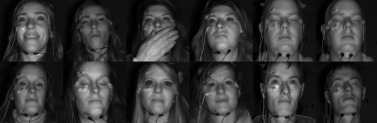
\includegraphics[scale=1]{gambar/3_1_5.jpg}
  % Keterangan gambar yang diinputkan
  \caption{Dataset DROZY}
  % Label referensi dari gambar yang diinputkan
  \label{fig:Drozy}
\end{figure}


\subsection{Dataset UTA-RLDD}
\label{subsec:UTARLDD}

Dataset RLDD terdiri dari sekitar 30 jam video RGB dari 50 partisipan yang sehat. Untuk setiap partisipan, kami memperoleh satu video untuk masing-masing dari tiga kelas yang berbeda: kewaspadaan, kewaspadaan rendah, dan kantuk, dengan total 50 video. Subjek penelitian adalah mahasiswa sarjana atau pascasarjana dan anggota staf yang berpartisipasi secara sukarela atau setelah menerima kredit tambahan dalam sebuah kursus. Semua partisipan berusia di atas 18 tahun.
Video diambil dari berbagai sudut yang berbeda di lingkungan dan latar belakang kehidupan nyata. Setiap video direkam sendiri oleh partisipan, menggunakan ponsel atau kamera web mereka. Kecepatan frame selalu kurang dari 30 fps, yang merupakan kecepatan frame yang diharapkan dari kamera tipikal yang digunakan oleh masyarakat umum.

\begin{figure} [H] \centering
  % Nama dari file gambar yang diinputkan
  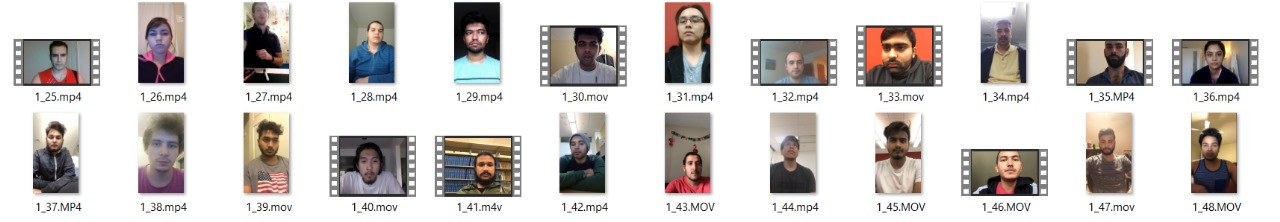
\includegraphics[width=\textwidth]{gambar/uta.jpg}
  % Keterangan gambar yang diinputkan
  \caption{Dataset UTA-RLDD}
  % Label referensi dari gambar yang diinputkan
  \label{fig:UTARLDD}
\end{figure}


\subsection{Peralatan dan Perangkat}
Pada Penelitian ini digunakan perangkat laptop dengan spesifikasi RAM 16 GB, Processor AMD Ryzen 5 4600H, graphic card NVIDIA GeForce GTX 1650, selain itu untuk melakukan training model dan lain lain digunakan Kaggle dan PyCharm. PyCharm adalah Integrated Development Environment (IDE) yang digunakan untuk pemrograman Python. Kaggle digunakan untuk meningkatkan keterampilan data untuk mendapatkan model, sedangkan PyCharm digunakan untuk Preprocessing data video yang akan digunakan.
